\section{Результаты экспериментов}

\subsection{Использование TCP для передачи данных}

В качестве точки отсчета в настоящей работе выступает метод межпроцессного взаимодействия на основе TCP, используемый посредством сокетов \textbf{TBD: ссылка на определение и на раздел диссертации} \ref{chapter31:PureTCP}. Гистограмма временной задержки на передачу данных для данного метода приведена на Рисунке \ref{chapter41:FigPureTCP}.

\begin{figure}[!h]
\caption{Гистограмма временной задержки на передачу данных между процессами при использовании TCP}
\label{chapter41:FigPureTCP}
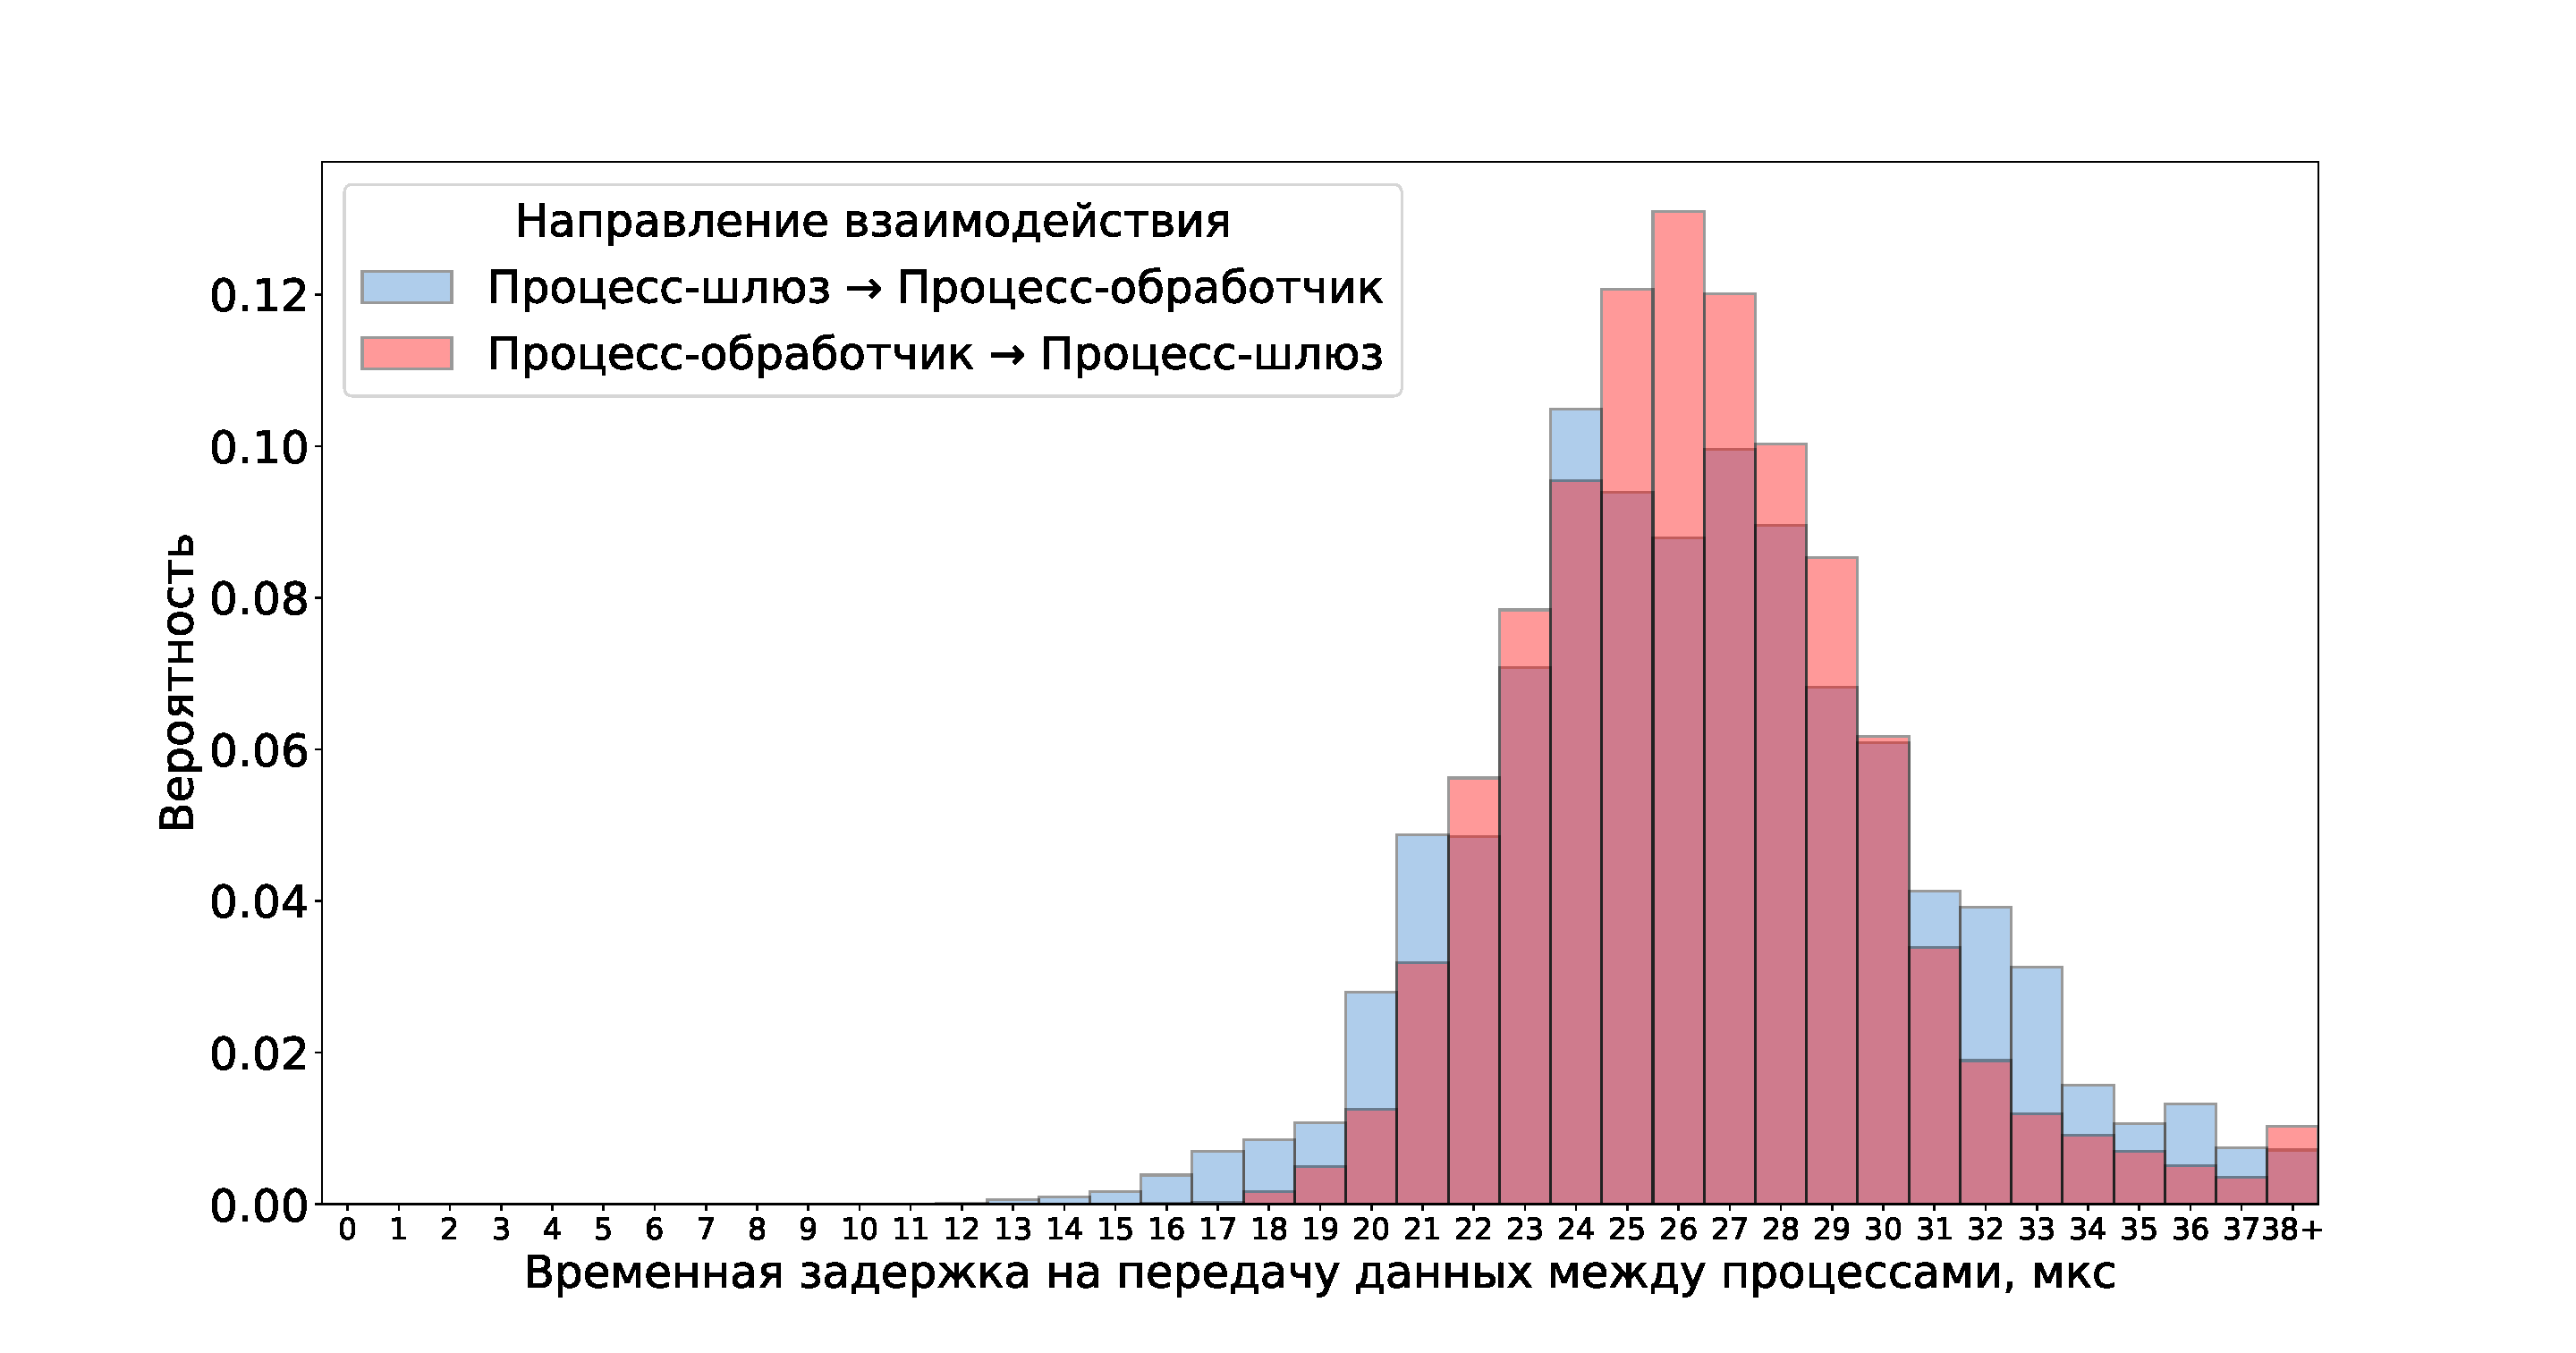
\includegraphics[width=\textwidth]{../../graphics/hist/PureTCP}
\end{figure}

В данном эксперименте симулятор отправляет серию заявок каждые \textit{10 $\pm$ 4 мс} с интервалом \textit{50 $\pm$ 26 мкс}  с коэффициентом доверия 95\%.

В Таблице \ref{chapter41:TablePureTCP} приведены основные временные характеристики данного метода. Временная задержка на передачу данных в обоих направлениях имеет схожие значения.

\begin{table}[!h]
\caption{Основные показатели временной задержки на передачу данных для метода на основе TCP}\label{chapter41:TablePureTCP}
\centering
\begin{tabular}{|l|c|c|}
\hline
\begin{tabular}[c]{@{}l@{}}Направление\\ взаимодействия/\\ Показатель\end{tabular} & \multicolumn{1}{l|}{\begin{tabular}[c]{@{}l@{}}Процесс-шлюз $\rightarrow$\\ Процесс-обработчик\end{tabular}} & \multicolumn{1}{l|}{\begin{tabular}[c]{@{}l@{}}Процесс-обработчик $\rightarrow$\\ Процесс-шлюз\end{tabular}} \\ \hline
min(t), мкс & 9 & 13 \\ \hline
M(t) $\pm$ 95\%, мкс & 27.5 $\pm$ 8.5 & 28 $\pm$ 7 \\ \hline
max(t), мс & 2.1 & 9.2 \\ \hline
\begin{tabular}[c]{@{}l@{}}$\delta$ между\\ сериями, мс\end{tabular} & 10 $\pm$ 4 & 10 $\pm$ 4 \\ \hline
\begin{tabular}[c]{@{}l@{}}$\delta$ между\\ заявками в серии, мкс\end{tabular} & 50 $\pm$ 26 & 87 $\pm$ 32 \\ \hline
\end{tabular}
\end{table}

\subsection{Использование разделяемой памяти для передачи данных}

\subsubsection{Использование TCP для оповещения о появлении данных}

В данном эксперименте симулятор отправляет серию заявок каждые \textit{10 $\pm$ 4 мс} с интервалом \textit{50 $\pm$ 27 мкс} с коэффициентом доверия 95\%.

В данном подразделе приведены данные об экспериментах с методом межпроцессного взаимодействия, описанным в Разделе \ref{chapter31:SignalTCP}.

\begin{figure}[!h]
\caption{Гистограмма временной задержки на передачу данных между процессами при использовании разделяемой памяти для передачи данных и TCP для оповещения о появлении данных в ней}
\label{chapter41:FigSignalTCP}
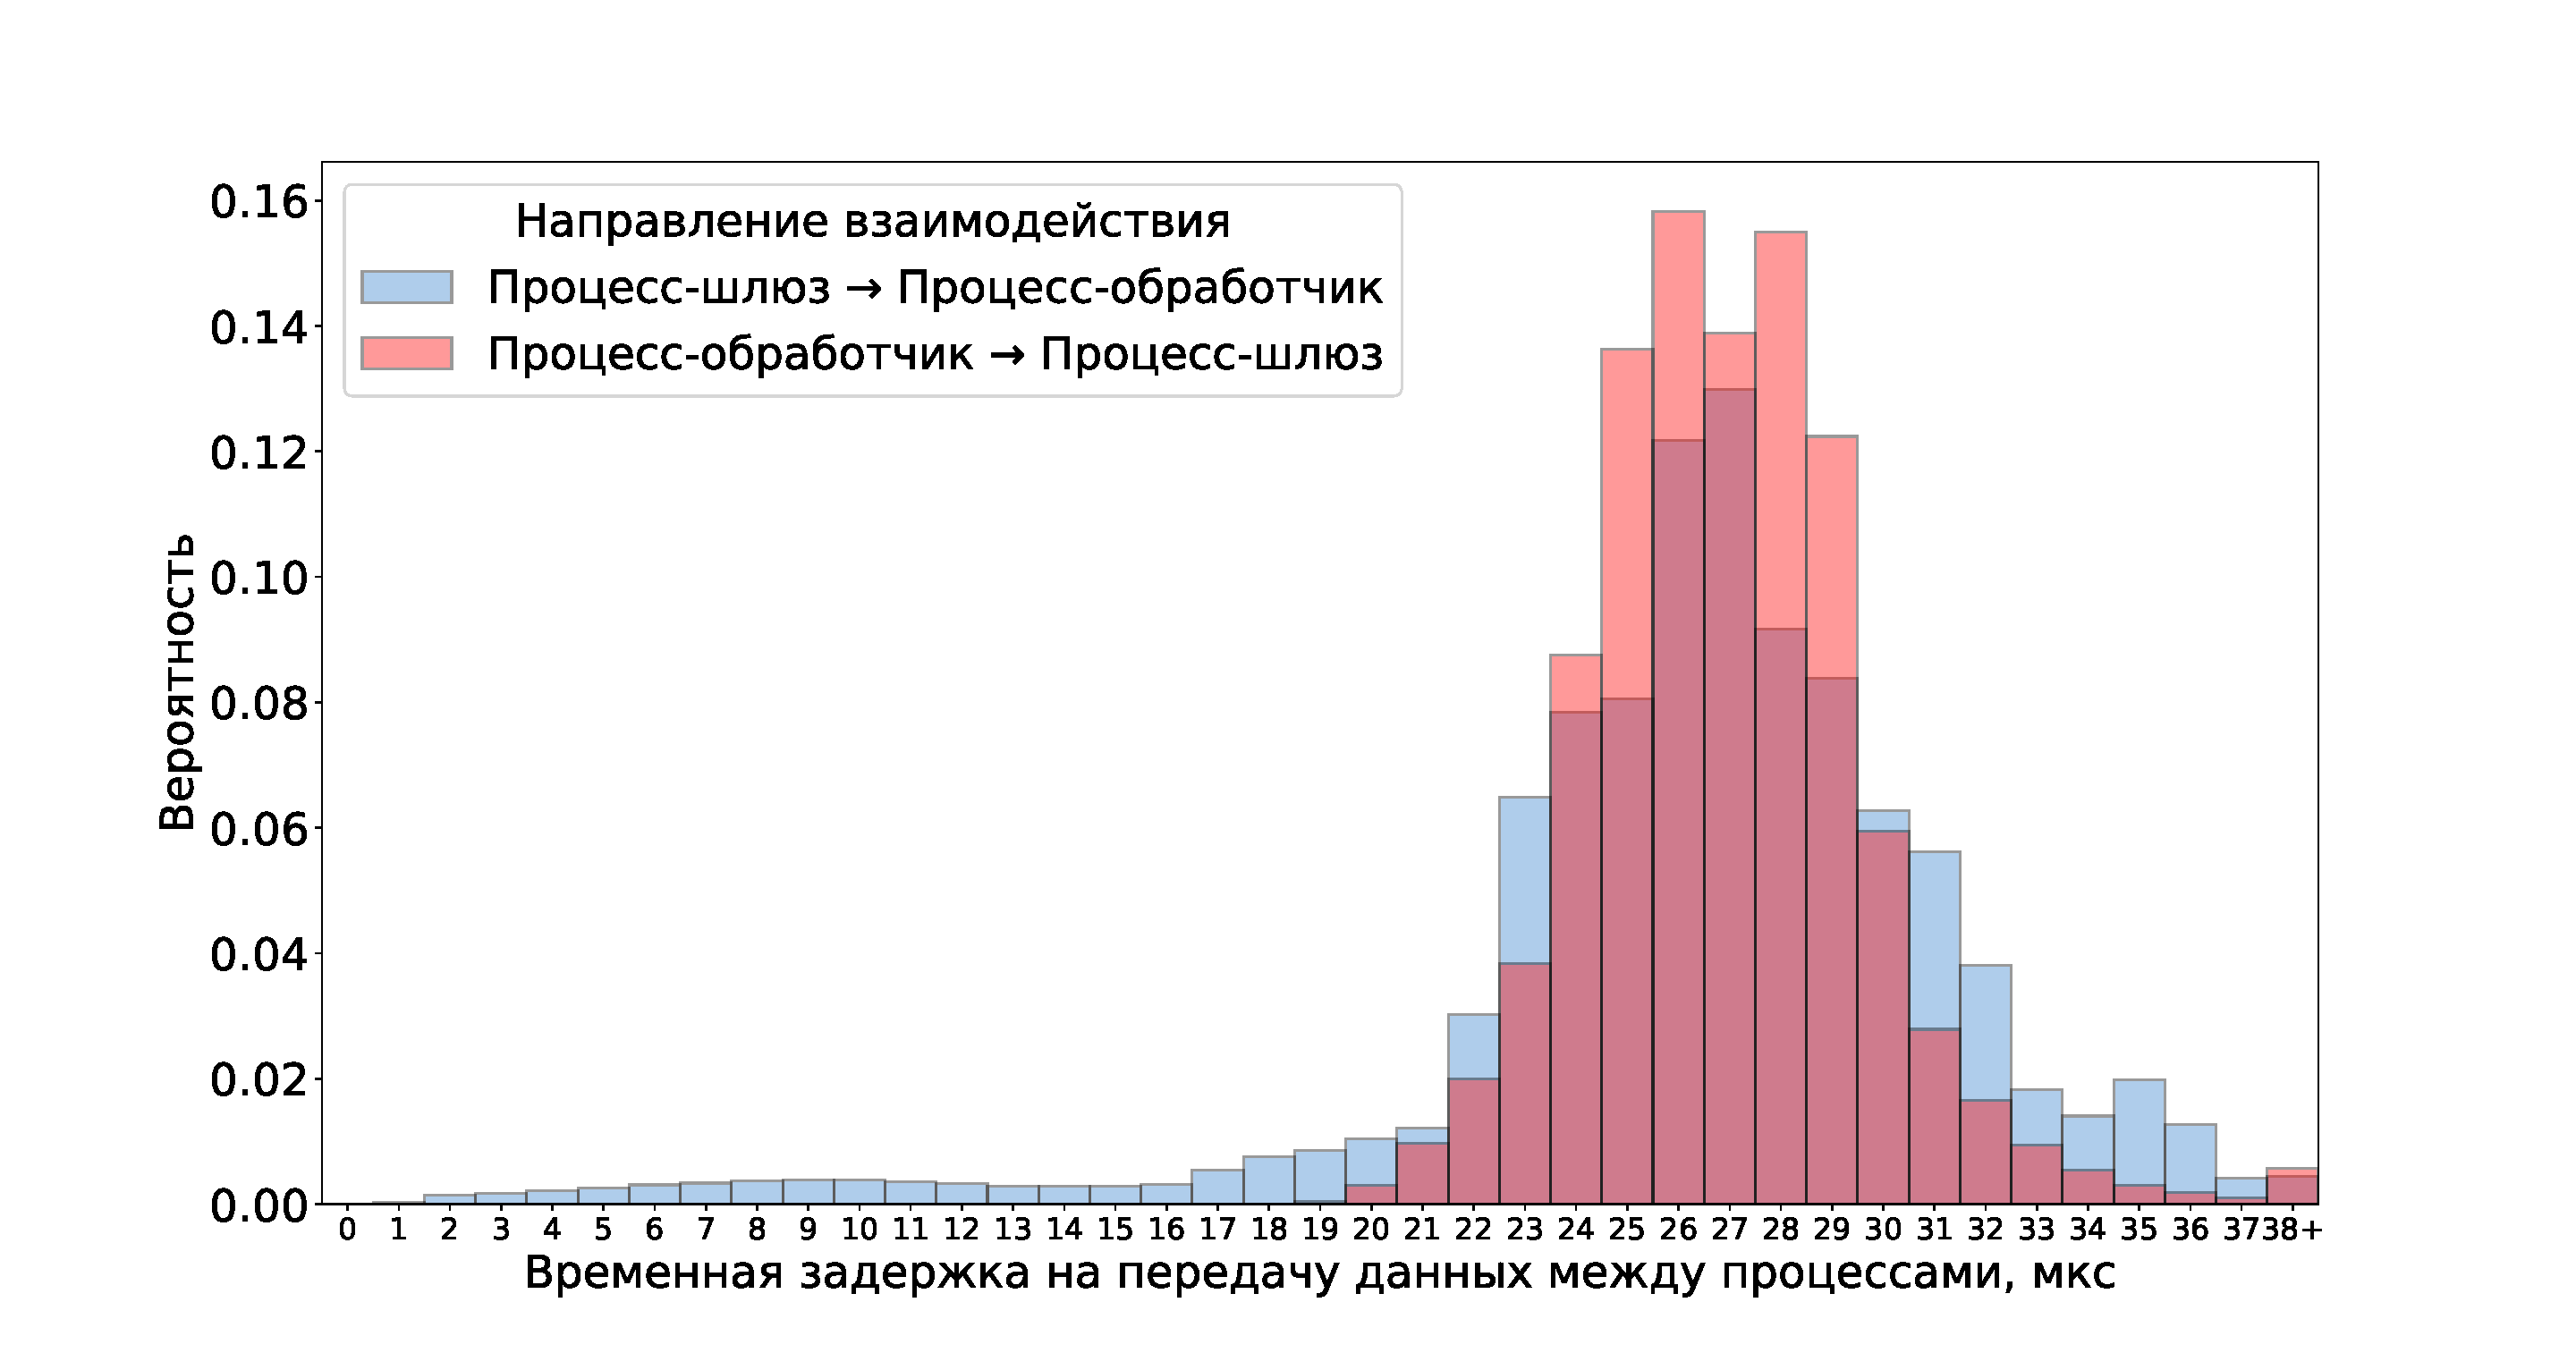
\includegraphics[width=\textwidth]{../../graphics/hist/SignalTCP}
\end{figure}

В Таблице \ref{chapter41:TableSignalTCP} приведены основные временные характеристики данного метода. Межпроцессное взаимодействие в сторону процесса-обработчика работает быстрее, т.к. в среднем время обслуживания заявок в процессе-обработчике заметно меньше (см. Рисунок \ref{chapter41:EngineLatency}), чем скорость поступления новых заявок, что позволяет использовать оптимизацию, описанную в Разделе \ref{chapter31:SharedMemoryOptimization} \textbf{TBD: сослаться на оптимизацию про отсутствие необходимости отправки новых сигналов, когда старые еще не были обработаны.}.

\begin{table}[!h]
\caption{Основные показатели временной задержки на передачу данных для метода, использующего разделяемую памяти для передачи данных и TCP для оповещения о появлении данных в ней}\label{chapter41:TableSignalTCP}
\centering
\begin{tabular}{|l|c|c|}
\hline
\begin{tabular}[c]{@{}l@{}}Направление\\ взаимодействия/\\ Показатель\end{tabular} & \multicolumn{1}{l|}{\begin{tabular}[c]{@{}l@{}}Процесс-шлюз $\rightarrow$\\ Процесс-обработчик\end{tabular}} & \multicolumn{1}{l|}{\begin{tabular}[c]{@{}l@{}}Процесс-обработчик $\rightarrow$\\ Процесс-шлюз\end{tabular}} \\ \hline
min(t), мкс & 1 & 3 \\ \hline
M(t) $\pm$ 95\%, мкс & 22.5 $\pm$ 12.5 & 27.5 $\pm$ 5.5 \\ \hline
max(t), мс & 3 & 9ю8 \\ \hline
\begin{tabular}[c]{@{}l@{}}$\delta$ между\\ сериями, мс\end{tabular} & 10 $\pm$ 4 & 10 $\pm$ 4 \\ \hline
\begin{tabular}[c]{@{}l@{}}$\delta$ между\\ заявками в серии, мкс\end{tabular} & 50 $\pm$ 27 & 87 $\pm$ 32 \\ \hline
\end{tabular}
\end{table}

\subsubsection{Использование мультиплексора в разделяемой памяти для оповещения о появлении данных}

В данном подразделе приведены данные об экспериментах с методом межпроцессного взаимодействия, описанным в Разделе \ref{chapter31:SignalTCP}.

\paragraph{Блокирующие методы}

В блокирующих методах поток мультиплексора событий использует примитив \textit{futex} \textbf{Может, сослаться на определение futex?} для пассивного ожидания новых сигналов (см. Раздел \ref{chapter31:BlockingMux}).

\subparagraph{Диспетчеризация и обработка соединений по модели "Полусинхронный/Полуреактивный"}

В данном эксперименте симулятор отправляет серию заявок каждые \textit{10 $\pm$ 4 мс} с интервалом \textit{51 $\pm$ 28 мкс} с коэффициентом доверия 95\%.

В данном подразделе приведены данные об экспериментах с методом межпроцессного взаимодействия, описанным в Разделе \ref{chapter31:BlockingHSHA}.

В Таблице \ref{chapter41:TableBlockingHSHA} приведены основные временные характеристики данного метода. \textbf{TBD}

На Рисунке \ref{chapter41:FigBlockingHSHA} приведена плотность вероятности временной задержки на передачу данных для данного метода.

\begin{figure}[!h]
\caption{Гистограмма временной задержки на передачу данных между процессами для метода, использующего разделяемую память для передачи данных, блокирующий мультиплексор в разделяемой памяти и модель ''Полусинхронный/Полуреактивный`` при обслуживании заявок}
\label{chapter41:FigBlockingHSHA}
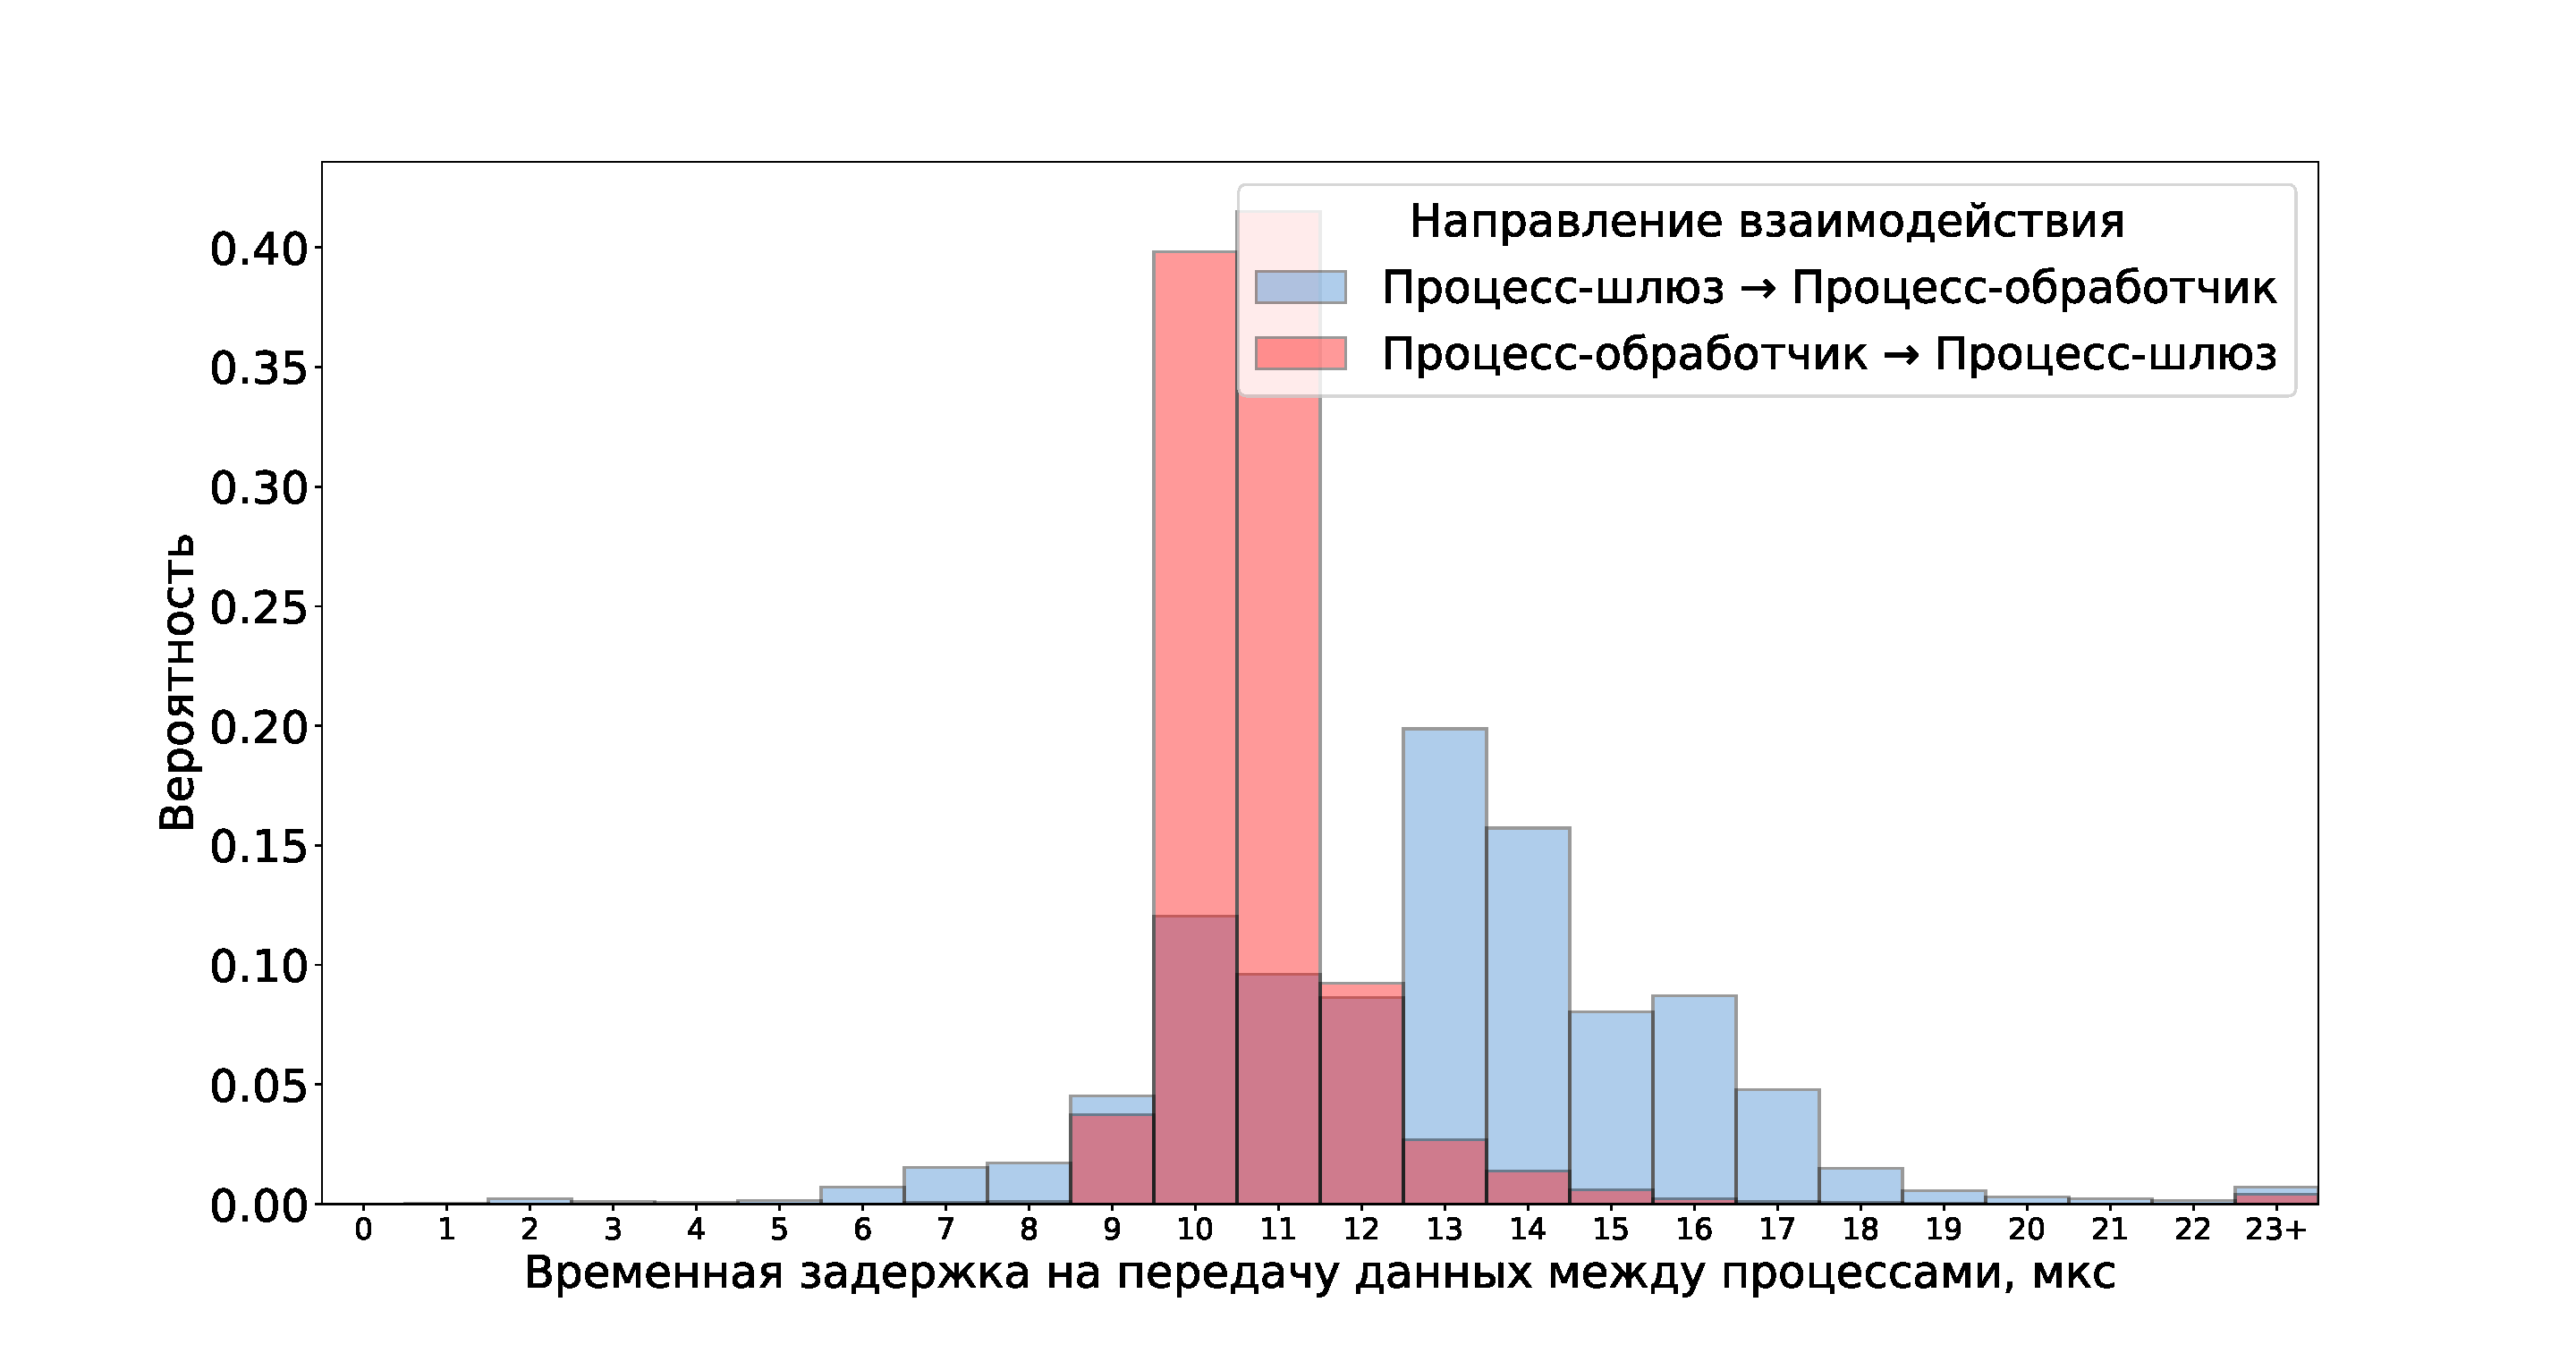
\includegraphics[width=\textwidth]{../../graphics/hist/BlockingHSHA}
\end{figure}
%
%В Таблице \ref{chapter41:TableBlockingHSHA} приведены основные временные характеристики данного метода. Межпроцессное взаимодействие в сторону процесса-обработчика работает быстрее, т.к. в среднем время обслуживания заявок в процессе-обработчике заметно меньше (см. Рисунок \ref{chapter41:EngineLatency}), чем скорость поступления новых заявок, что позволяет использовать оптимизацию, описанную в Разделе \ref{chapter31:SharedMemoryOptimization} \textbf{TBD: сослаться на оптимизацию про отсутствие необходимости отправки новых сигналов, когда старые еще не были обработаны.}.

\begin{table}[!h]
\caption{Основные показатели временной задержки на передачу данных между процессами для метода, использующего разделяемую память для передачи данных, блокирующий мультиплексор в разделяемой памяти и модель ''Полусинхронный/Полуреактивный`` при обслуживании заявок}\label{chapter41:TableBlockingHSHA}
\centering
\begin{tabular}{|l|c|c|}
\hline
\begin{tabular}[c]{@{}l@{}}Направление\\ взаимодействия/\\ Показатель\end{tabular} & \multicolumn{1}{l|}{\begin{tabular}[c]{@{}l@{}}Процесс-шлюз $\rightarrow$\\ Процесс-обработчик\end{tabular}} & \multicolumn{1}{l|}{\begin{tabular}[c]{@{}l@{}}Процесс-обработчик $\rightarrow$\\ Процесс-шлюз\end{tabular}} \\ \hline
min(t), мкс & 1 & 3 \\ \hline
M(t) $\pm$ 95\%, мкс & 12.5 $\pm$ 5.5 & 11.5 $\pm$ 2.5 \\ \hline
max(t), мс & 6.9 & 11.6 \\ \hline
\begin{tabular}[c]{@{}l@{}}$\delta$ между\\ сериями, мс\end{tabular} & 10 $\pm$ 4 & 10 $\pm$ 4 \\ \hline
\begin{tabular}[c]{@{}l@{}}$\delta$ между\\ заявками в серии, мкс\end{tabular} & 51 $\pm$ 28 & 91 $\pm$ 36 \\ \hline
\end{tabular}
\end{table}

\subparagraph{Диспетчеризация и обработка соединений по модели "Лидер/Последователи"}

В данном эксперименте симулятор отправляет серию заявок каждые \textit{8.4 $\pm$ 5.3 мс} с интервалом \textit{52 $\pm$ 28 мкс} с коэффициентом доверия 95\%.

В данном подразделе приведены данные об экспериментах с методом межпроцессного взаимодействия, описанным в Разделе \ref{chapter31:BlockingLF}.

В Таблице \ref{chapter41:TableBlockingLF} приведены основные временные характеристики данного метода. \textbf{TBD}

На Рисунке \ref{chapter41:FigBlockingLF} приведена плотность вероятности временной задержки на передачу данных для данного метода.

\begin{figure}[!h]
\caption{Гистограмма временной задержки на передачу данных между процессами для метода, использующего разделяемую память для передачи данных, блокирующий мультиплексор в разделяемой памяти и модель ''Лидер/Последователи`` при обслуживании заявок}
\label{chapter41:FigBlockingLF}
\includegraphics[width=\textwidth]{../../graphics/hist/BlockingLF}
\end{figure}
%
%В Таблице \ref{chapter41:TableBlockingHSHA} приведены основные временные характеристики данного метода. Межпроцессное взаимодействие в сторону процесса-обработчика работает быстрее, т.к. в среднем время обслуживания заявок в процессе-обработчике заметно меньше (см. Рисунок \ref{chapter41:EngineLatency}), чем скорость поступления новых заявок, что позволяет использовать оптимизацию, описанную в Разделе \ref{chapter31:SharedMemoryOptimization} \textbf{TBD: сослаться на оптимизацию про отсутствие необходимости отправки новых сигналов, когда старые еще не были обработаны.}.

\begin{table}[!h]
\caption{Основные показатели временной задержки на передачу данных между процессами для метода, использующего разделяемую память для передачи данных, блокирующий мультиплексор в разделяемой памяти и модель ''Лидер/Последователи`` при обслуживании заявок}\label{chapter41:TableBlockingLF}
\centering
\begin{tabular}{|l|c|c|}
\hline
\begin{tabular}[c]{@{}l@{}}Направление\\ взаимодействия/\\ Показатель\end{tabular} & \multicolumn{1}{l|}{\begin{tabular}[c]{@{}l@{}}Процесс-шлюз $\rightarrow$\\ Процесс-обработчик\end{tabular}} & \multicolumn{1}{l|}{\begin{tabular}[c]{@{}l@{}}Процесс-обработчик $\rightarrow$\\ Процесс-шлюз\end{tabular}} \\ \hline
min(t), мкс & 1 & 2 \\ \hline
M(t) $\pm$ 95\%, мкс & 11.5 $\pm$ 6.5 & 9.5 $\pm$ 1.5 \\ \hline
max(t), мс & 2.4 & 9.5 \\ \hline
\begin{tabular}[c]{@{}l@{}}$\delta$ между\\ сериями, мс\end{tabular} & 8.4 $\pm$ 5.3 & 8.4 $\pm$ 5.3 \\ \hline
\begin{tabular}[c]{@{}l@{}}$\delta$ между\\ заявками в серии, мкс\end{tabular} & 52 $\pm$ 29 & 90 $\pm$ 35 \\ \hline
\end{tabular}
\end{table}





\paragraph{Неблокирующий метод}

В неблокирующем методе поток мультиплексора событий метод активного ожидания новых сигналов (см. Раздел \ref{chapter31:NonBlockingMux}). В данном параграфе рассматривается исключительно модель обслуживания заявок ''Лидер/Последователи`` т.к. в параграфе выше она показала лучшие результаты по сравнению с моделью ''Полусинхронный/Полуреактивный``.

\subparagraph{Диспетчеризация и обработка соединений по модели "Лидер/Последователи"}

В данном эксперименте симулятор отправляет серию заявок каждые \textit{7.4 $\pm$ 5.9 мс} с интервалом \textit{55 $\pm$ 32 мкс} с коэффициентом доверия 95\%.

В данном подразделе приведены данные об экспериментах с методом межпроцессного взаимодействия, описанным в Разделе \ref{chapter31:NonBlockingLF}.

В Таблице \ref{chapter41:TableNonBlockingLF} приведены основные временные характеристики данного метода. \textbf{TBD}

На Рисунке \ref{chapter41:FigNonBlockingLF} приведена плотность вероятности временной задержки на передачу данных для данного метода.

\begin{figure}[!h]
\caption{Гистограмма временной задержки на передачу данных между процессами для метода, использующего разделяемую память для передачи данных, блокирующий мультиплексор в разделяемой памяти и модель ''Лидер/Последователи`` при обслуживании заявок}
\label{chapter41:FigNonBlockingLF}
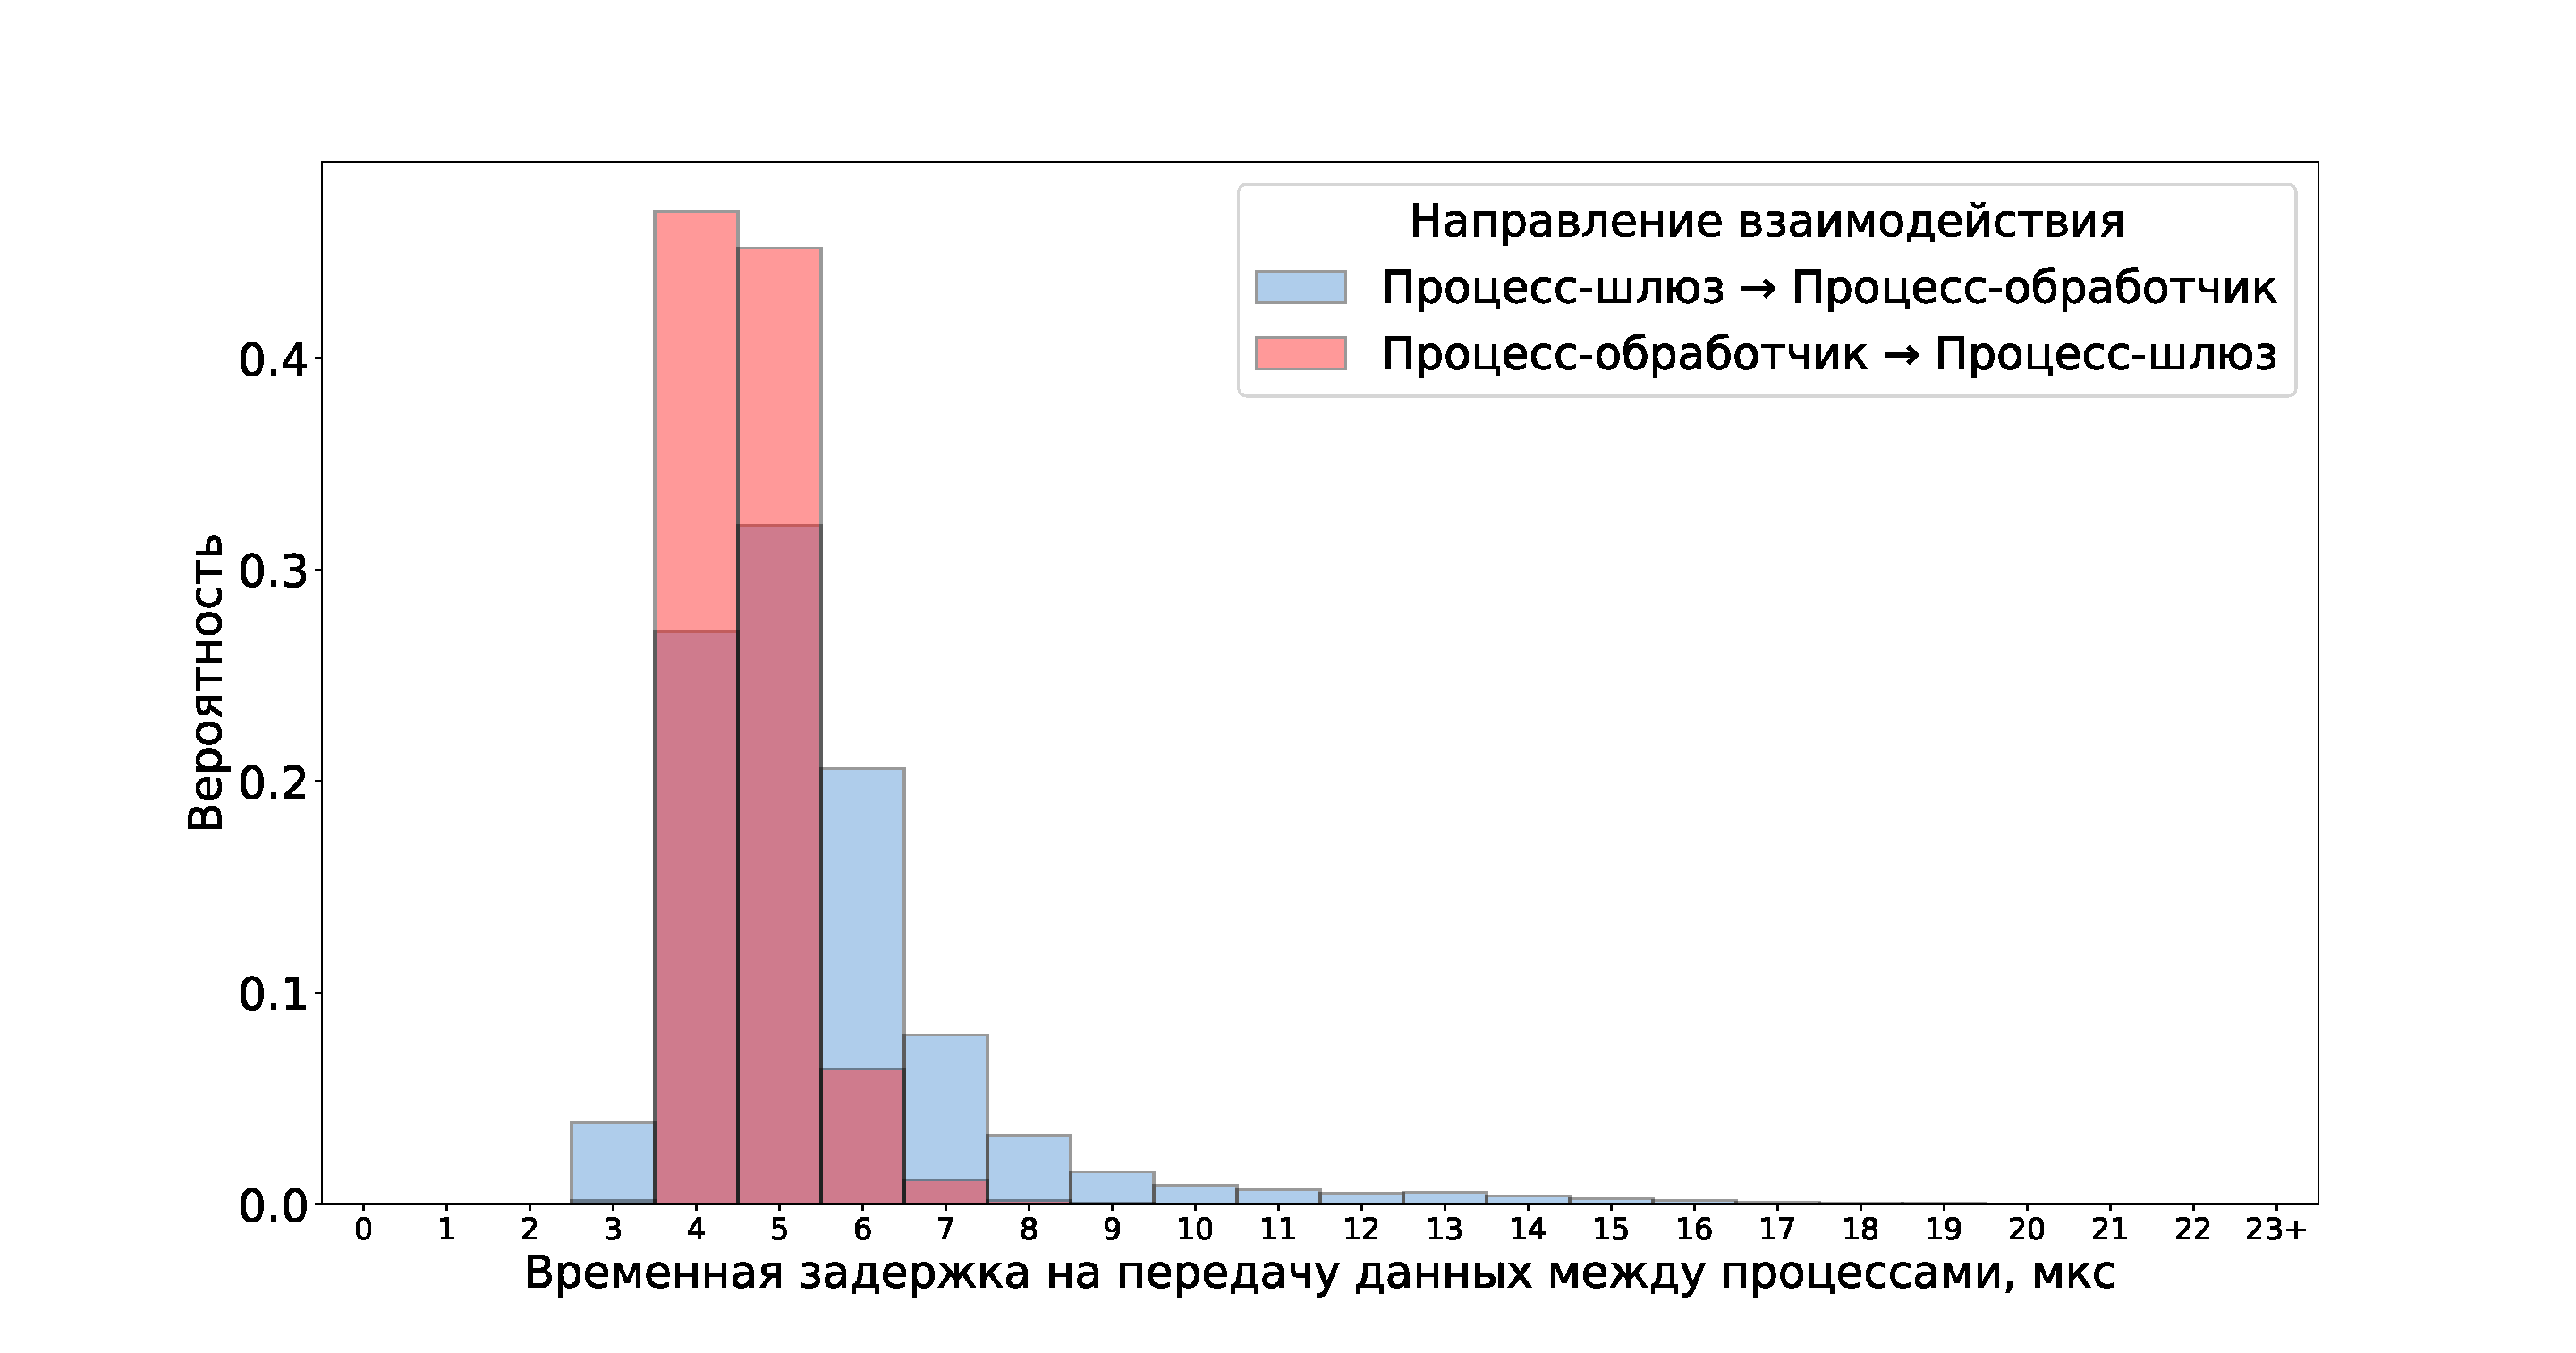
\includegraphics[width=\textwidth]{../../graphics/hist/NonBlockingLF}
\end{figure}
%
%В Таблице \ref{chapter41:TableBlockingHSHA} приведены основные временные характеристики данного метода. Межпроцессное взаимодействие в сторону процесса-обработчика работает быстрее, т.к. в среднем время обслуживания заявок в процессе-обработчике заметно меньше (см. Рисунок \ref{chapter41:EngineLatency}), чем скорость поступления новых заявок, что позволяет использовать оптимизацию, описанную в Разделе \ref{chapter31:SharedMemoryOptimization} \textbf{TBD: сослаться на оптимизацию про отсутствие необходимости отправки новых сигналов, когда старые еще не были обработаны.}.

\begin{table}[!h]
\caption{Основные показатели временной задержки на передачу данных между процессами для метода, использующего разделяемую память для передачи данных, блокирующий мультиплексор в разделяемой памяти и модель ''Лидер/Последователи`` при обслуживании заявок}\label{chapter41:TableNonBlockingLF}
\centering
\begin{tabular}{|l|c|c|}
\hline
\begin{tabular}[c]{@{}l@{}}Направление\\ взаимодействия/\\ Показатель\end{tabular} & \multicolumn{1}{l|}{\begin{tabular}[c]{@{}l@{}}Процесс-шлюз $\rightarrow$\\ Процесс-обработчик\end{tabular}} & \multicolumn{1}{l|}{\begin{tabular}[c]{@{}l@{}}Процесс-обработчик $\rightarrow$\\ Процесс-шлюз\end{tabular}} \\ \hline
min(t), мкс & 1 & 3 \\ \hline
M(t) $\pm$ 95\%, мкс & 7 $\pm$ 4 & 5 $\pm$ 1 \\ \hline
max(t), мс & 8.5 & 0.003 \\ \hline
\begin{tabular}[c]{@{}l@{}}$\delta$ между\\ сериями, мс\end{tabular} & 7.4 $\pm$ 5.9 & 7.4 $\pm$ 5.9 \\ \hline
\begin{tabular}[c]{@{}l@{}}$\delta$ между\\ заявками в серии, мкс\end{tabular} & 58 $\pm$ 35 & 167 $\pm$ 113 \\ \hline
\end{tabular}
\end{table}